%%%%%%%%%%%%%%%%%%%%%%%%%%%%%%%%%%%%%%%%%%%%%%%%%%%%
%%											  	 %%
%% Author : Andreas Apostolatos               	 %%
%%											  	 %%
%% e-mail : andreas.apostolatos@tum.de		   	 %%
%%											  	 %%
%% 09_Appendix.tex					  	   	  	 %%
%%											  	 %%
%%%%%%%%%%%%%%%%%%%%%%%%%%%%%%%%%%%%%%%%%%%%%%%%%%%%
\section{Appendix}

Here all theorems or general concepts that have been used in the report and seek further explanation should be placed.\\[6pt]
Note that the references come before the appendix. The references need to be written in .bib format, see the attached file references.bib. Then you should compile three times the document with bibTex and other three times with LatexMk (or simply Latex) and they should normally appear into the text automatically.\\[6pt]
%%%%%%%%%%%%%%%%%%%%%%%%%%%%%% MATLAB %%%%%%%%%%%%%%%%%%%%%%%%%%%%%%%%
\subsection{Matlab Code} \label{section:appendix_matlab}
[INSERT CONTENT (AND SUBSECTIONS IF NEEDED)]

%%%%%%%%%%%%%%%%%%%%%%%%%%%%%%% GiD %%%%%%%%%%%%%%%%%%%%%%%%%%%%%%%%%%
\subsection{GiD GUI} \label{section:appendix_GiD}
The GiD user interface was modified as part of this assignment in order to facilitate the simple transfer of data from GiD to Matlab. All data entered by the user in GiD is contained within the \texttt{.dat} file generated by GiD. Matlab reads the \texttt{.dat} file as an input for the calculations. Please note that only the functionality

%%%%%%%%%%%%%%%%%%%%%%%%%%%% GiD - Setup %%%%%%%%%%%%%%%%%%%%%%%%%%%%%
\subsubsection{Setup}
GiD is equipped with various \texttt{problem types}, which contain the commands to customize the user interface. All of the enhancements made to GiD are within the \texttt{Matlab} problem type. To select this, under the \texttt{Data} heading, click \texttt{Problem type} $\rightarrow$ \texttt{matlab}. See Figure \ref{fig:Matlabproblemtype}.

\begin{figure}[ht]
  \centering
  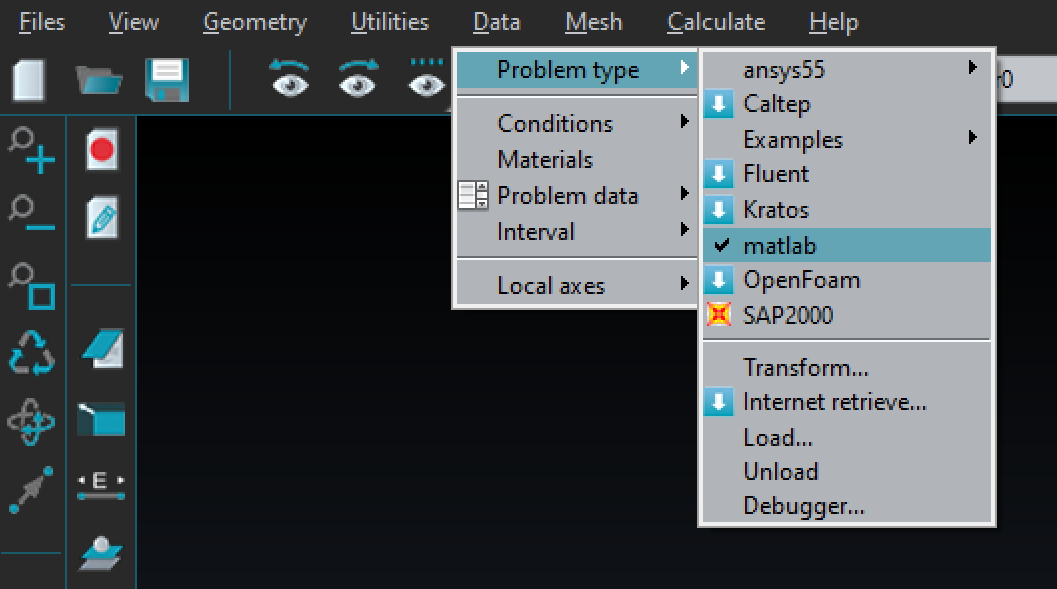
\includegraphics[width=80mm]{images/GiD_probtype.png}
  \caption{\texttt{Matlab} problem type selection}
  \label{fig:Matlabproblemtype}
\end{figure}
Next, create a geometry using the \texttt{geometry} $\rightarrow$ \texttt{create} menu.

%%%%%%%%%%%%%%%%%%%%%%% GiD - boundary conditions %%%%%%%%%%%%%%%%%%%%%%%%
\subsubsection{Boundary Conditions}
Once the geometry is created, the user must apply boundary conditions in order to constrain the model. Click \texttt{Data} $\rightarrow$ \texttt{Conditions} $\rightarrow$ \texttt{Constraints}, and the menu shown in Figure \ref{fig:GiDConstraints} will appear. For a plane stress problem, only $x$ and $y$ constraints should be applied. In the example shown in this paper, a value of 0.0 was used for each.\\[6pt]
\begin{figure}[ht]
  \centering
  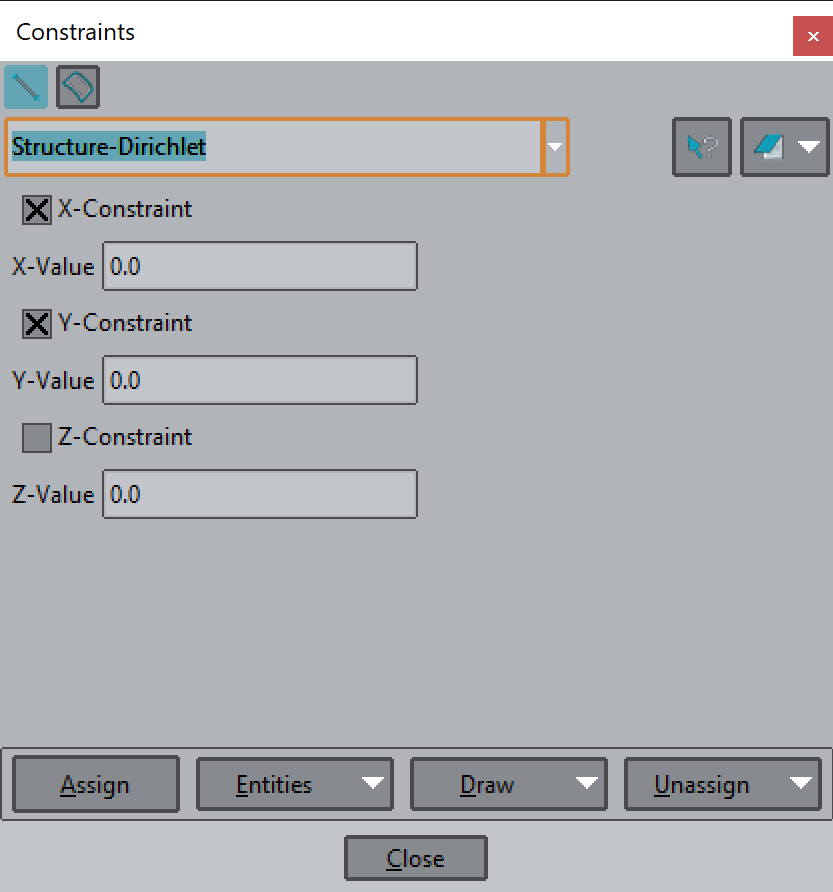
\includegraphics[width=60mm]{images/GiD_constraints.png}
  \caption{constraints menu}
  \label{fig:GiDConstraints}
\end{figure}
Next, click \texttt{Assign} and then click on the edge of the model to apply the desired constraint.

%%%%%%%%%%%%%%%%%%%%%%%%%%%%% GiD - loads %%%%%%%%%%%%%%%%%%%%%%%%%%%%%%%%%
\subsubsection{Loads}
The first modification made to GiD was to allow for the application of point loads. The primary purpose for this was to simplify equation \ref{eqn:responsefctderivative}. The term $\dv{\textbf{P}}{x_i}$ represents the change in the force vector, $\textbf{P}$, with respect to the design variables, $x_i$. This term vanishes if the force vector is constant with respect to the design variables, which is the case when a point load is applied. This simplified equation would make initial implementation and validation of the numerical and analytical sensitivity equations a bit easier\\[6pt]
The ability to apply a distributed load was already contained within the \texttt{Matlab} problem type. To apply a load, simply click on the \texttt{Data} heading, then \texttt{conditions} $\rightarrow$ \texttt{loads}. The menu shown in Figure \ref{fig:GiDLoadsDist} will appear. There are only two actions that need to be taken. First, select the proper function handle. There is a \texttt{computeConstantVerticalLoad} and a \texttt{computeConstantHorizontalLoad} option. They correspond to functions within the Matlab code hierarchy that assign a constant vertical or horizontal load, respectively. In these functions, the user can input the desired load magnitude. Second, click \texttt{Assign}. Then, select the edge of the structure on which to apply the distributed load.

\begin{figure}[ht]
  \centering
  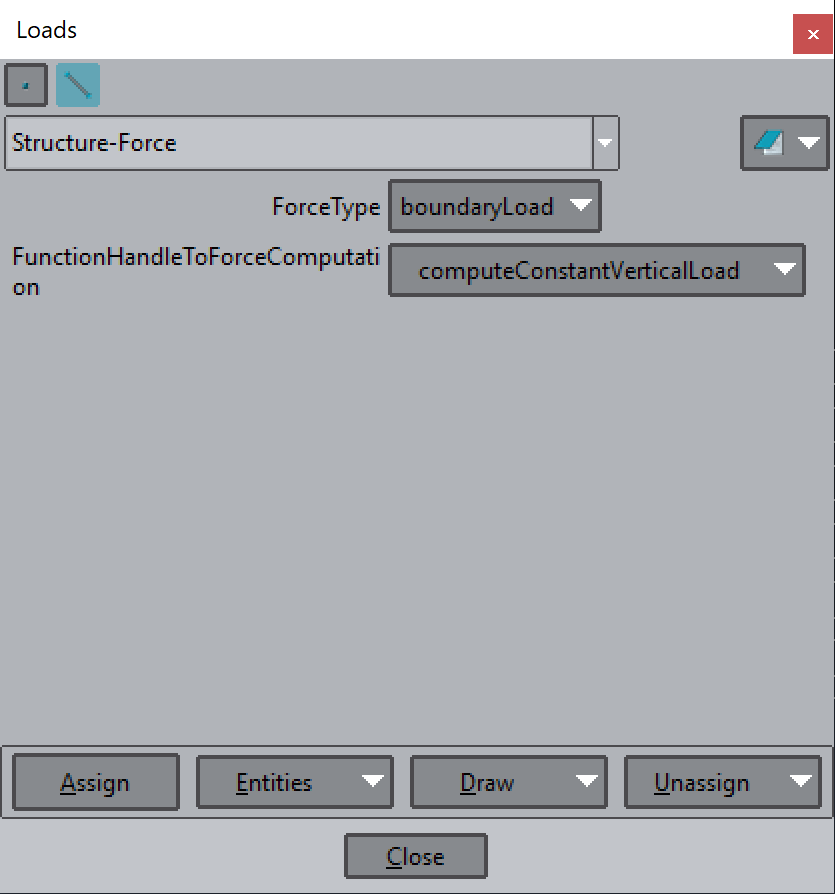
\includegraphics[width=60mm]{images/GiD_loads_dist.png}
  \caption{distributed loads menu}
  \label{fig:GiDLoadsDist}
\end{figure}

In addition to being able to apply a distributed load, the user can apply a point load. This is the functionality added to aid the development of the sensitivity analysis program. The associated menu is also under \texttt{Data} $\rightarrow$ \texttt{Conditions} $\rightarrow$ \texttt{Loads}. Simply click on the symbol in the upper left of the menu to toggle between point and distributed loads. See Figure \ref{fig:GiDLoadsPoint}. Before applying a point load, the mesh must first be generated! The most simple way to generate a mesh in GiD is to click \texttt{Mesh} $\rightarrow$ \texttt{Generate mesh}. Then, enter the desired element size. \textbf{Note:} too small of a mesh size will cause long calculation times.

\begin{figure}[ht]
  \centering
  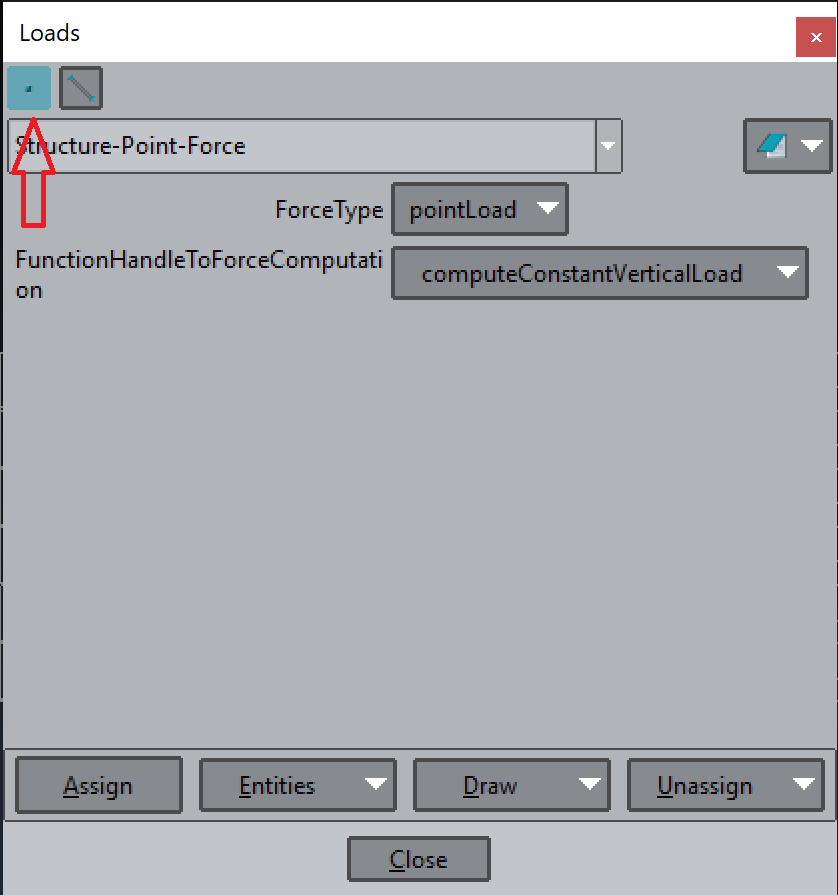
\includegraphics[width=60mm]{images/GiD_loads_point.png}
  \caption{point loads menu}
  \label{fig:GiDLoadsPoint}
\end{figure}
%%%%%%%%%%%%%%%%%%%%%%%% GiD - sensitivity analysis %%%%%%%%%%%%%%%%%%%%%%
\subsubsection{Sensitivity Analysis}
To define the sensitivity analysis parameters, click \texttt{Data} $\rightarrow$ \texttt{Problem Data} $\rightarrow$ \texttt{Sensitivity Analysis}. The menu shown in Figure \ref{fig:GiDSensAnalMenu} will appear. In the upper dropdown menu, the user can select the type of sensitivity analysis. The options are: \texttt{global}, \texttt{numerical adjoint}, and \texttt{analytical adjoint}. Exercise caution when selecting the global method - please ensure a relatively low number of nodes (less than ~200) is used. In the sensitivity analysis menu, the user can click the box next to the desired objective functions. Please note that currently, the von Mises stress objective function only works with the global method due to time constraints. Next, the user can select the finite differencing method: \texttt{forward}, \texttt{backward}, or \texttt{central}. Finally, the user can select the perturbation size. Based on the perturbation study discussed in section \ref{section:perturbationstudy}, a perturbation of $10^{-5}$ worked reliably.
\begin{figure}[ht]
  \centering
  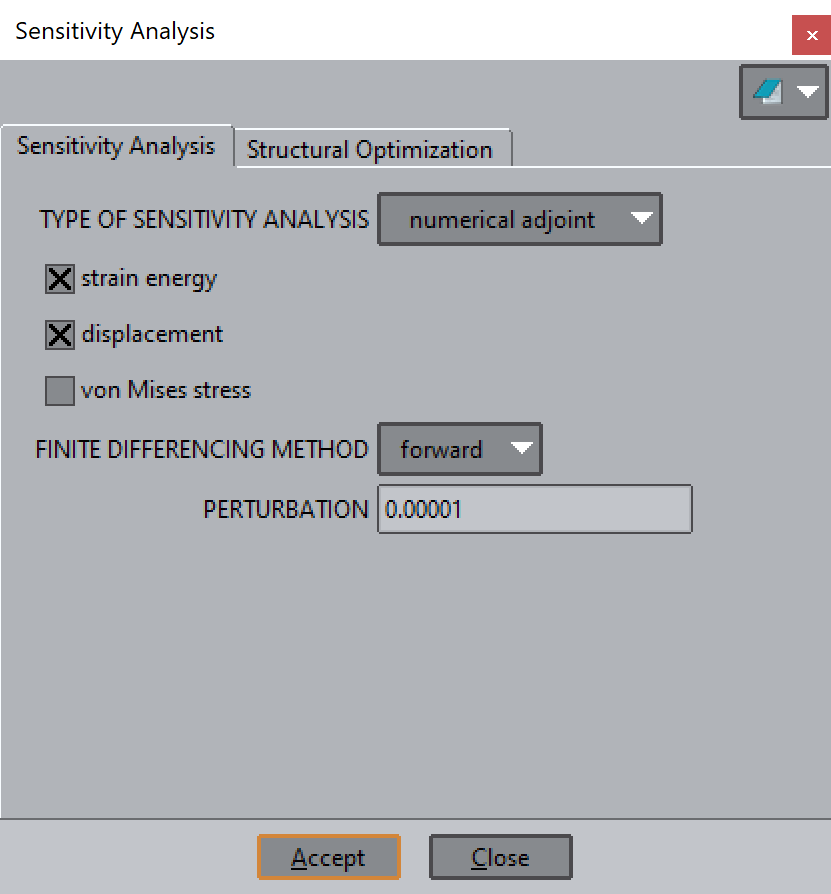
\includegraphics[width=60mm]{images/GiD_sens_analysis.png}
  \caption{sensitivity analysis menu}
  \label{fig:GiDSensAnalMenu}
\end{figure}

%%%%%%%%%%%%%%%%%%%%%%%%%%%% GiD - domains %%%%%%%%%%%%%%%%%%%%%%%%%
\subsubsection{Domains}
Next, click \texttt{Data} $\rightarrow$ \texttt{Conditions} $\rightarrow$ \texttt{Domains}. The menu shown in Figure \ref{fig:GiDDomainsMenu} will appear. In the dropdown menu, click \texttt{Structure-Nodes}, click \texttt{Assign}, select all nodes, and click \texttt{Finish}. Click \texttt{Structure-Elements} in the dropdown menu and perform the same steps.\\[6pt]
Next, parameters associated with the sensitivity analysis must be specified. These are also visible in Figure \ref{fig:GiDDomainsMenu} If a displacement sensitivity analysis is selected, then the user must specify which node(s) on which to perform the analysis. Simply click \texttt{Structure Nodes for Displacement Sensitivity}, \texttt{Assign}, and then select the appropriate node(s). The same steps apply to von Mises stress, except the user must select one or more elements instead of nodes. For a strain energy sensitivity analysis, no further action is needed since the analysis is applicable to the entire structure.
\begin{figure}[ht]
  \centering
  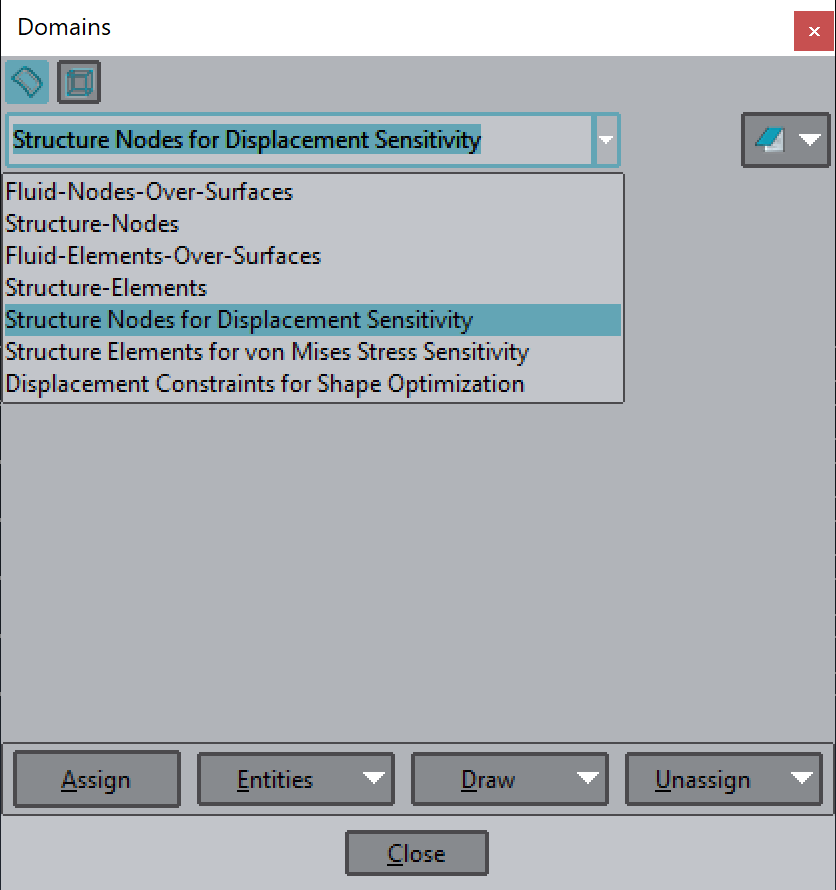
\includegraphics[width=60mm]{images/GiD_domains.png}
  \caption{domains menu}
  \label{fig:GiDDomainsMenu}
\end{figure}

%%%%%%%%%%%%%%%%%%%%%%%%%%%% GiD - materials %%%%%%%%%%%%%%%%%%%%%%%%%
\subsubsection{Material Properties}
Next, the user should input the material properties of the created geometry. Click \texttt{Data} $\rightarrow$ \texttt{Materials}, and the menu shown in Figure \ref{fig:GiDMaterialsMenu} will appear. Make sure to select \texttt{Structure} in the dropdown menu. Enter values appropriate for the type of material being simulated. Next, click \texttt{Assign} and draw a rectangle around all elements. Click \texttt{Finish}.

\begin{figure}[ht]
  \centering
  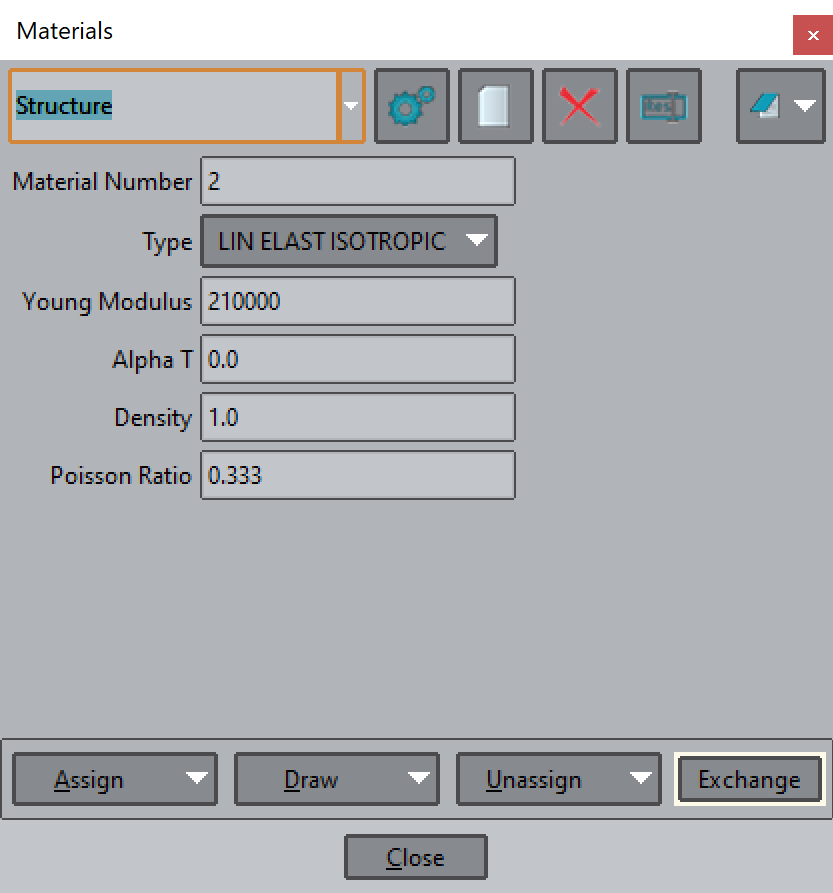
\includegraphics[width=60mm]{images/GiD_materials.png}
  \caption{material properties menu}
  \label{fig:GiDMaterialsMenu}
\end{figure}

%%%%%%%%%%%%%%%%%%%%%%%%%%%% GiD - optimization %%%%%%%%%%%%%%%%%%%%%%%%%
\subsubsection{Optimization}
If the user wants to execute the optimization algorithm, it can be found under \texttt{Data} $\rightarrow$ \texttt{Problem Data} $\rightarrow$ \texttt{Sensitivity Analysis}. Then select the \texttt{Structural Optimization} tab at the top of the menu. See Figure \ref{fig:GiDOptimizationMenu}. The user can specify the sensitivity analysis type, objective function, displacement direction, differencing method, perturbation, number of iterations, and factor of change. The recommended number of iterations is 10, and the recommended factor of change is 5. All other parameters have been discussed previously.

\begin{figure}[ht]
  \centering
  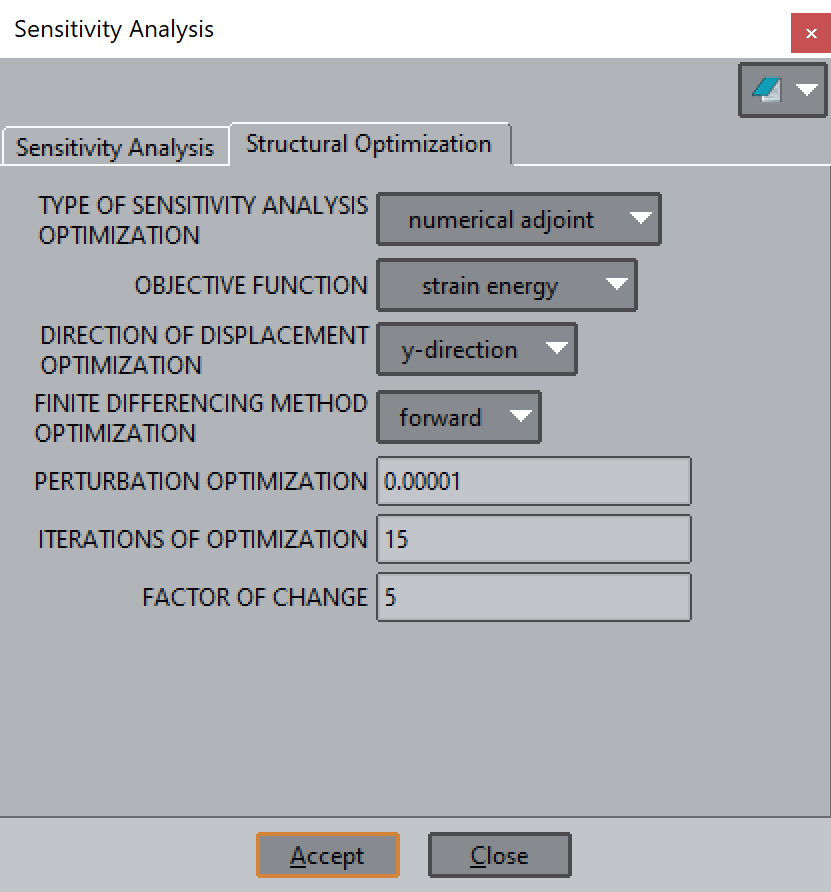
\includegraphics[width=60mm]{images/GiD_optimization.png}
  \caption{optimization menu}
  \label{fig:GiDOptimizationMenu}
\end{figure}

The optimization algorithm could be improved, as mentioned in Section \ref{section:optimization}. It is currently unstable if too many iterations are utilized; therefore, it is best to keep the iteration number at or below 10. The ideal factor of change will likely vary depending on the absolute size of the geometry created in GiD.

%%%%%%%%%%%%%%%%%%%%%%%%%%%% GiD - output %%%%%%%%%%%%%%%%%%%%%%%%%
\subsubsection{Output}
Now that all of the necessary information has been entered into GiD, ensure that the current file has been saved. Then, click \texttt{Calculate} $\rightarrow$ \texttt{Calculate}. This will generate a folder ending in \texttt{.gid}. There will be a \texttt{.dat} file within this folder. This file is what is read in from Matlab in the \texttt{main.m} driver file.  